% Presentación: aptitud solar FV y generación real en Colombia
% Compilar en Overleaf con pdfLaTeX. Subir este archivo y la carpeta figuras/ tal cual.
\documentclass[aspectratio=169,10pt]{beamer}

\usepackage[utf8]{inputenc}
\usepackage[T1]{fontenc}
\usepackage[spanish]{babel}
\usepackage{graphicx}
\usepackage{booktabs}
\usepackage{tabularx}
\usepackage{xcolor}
\urlstyle{same}

\usetheme[progressbar=frametitle, numbering=fraction, block=fill]{metropolis}
\usepackage{appendixnumberbeamer}
% Paleta rojo y negro (los nombres de las variables se conservan para no tocar el resto del archivo)
\definecolor{azul}{HTML}{1A1A1A}
\definecolor{azulclaro}{HTML}{F3D6D6}
\definecolor{naranja}{HTML}{C0141F}
\definecolor{gris}{HTML}{F4F4F4}
\setbeamercolor{normal text}{fg=azul}
\setbeamercolor{title}{fg=naranja}
\setbeamercolor{subtitle}{fg=azul}
\setbeamercolor{title separator}{fg=naranja}
\setbeamercolor{section title}{fg=azul}
\setbeamercolor{palette primary}{bg=azul, fg=white}
\setbeamercolor{itemize item}{fg=naranja}
\setbeamercolor{enumerate item}{fg=naranja}
\setbeamercolor{frametitle}{bg=azul, fg=white}
\setbeamercolor{progress bar}{fg=naranja, bg=azulclaro}
\setbeamercolor{alerted text}{fg=naranja}
\setbeamercolor{block title}{bg=azul, fg=white}
\setbeamercolor{block body}{bg=gris}
\setbeamercolor{block title alerted}{bg=naranja, fg=white}
\setbeamercolor{block body alerted}{bg=gris}
\setbeamercolor{background canvas}{bg=white}
\graphicspath{{figuras/}}

% Cifra grande para la diapositiva de resultados
\newcommand{\cifra}[2]{%
  \begin{minipage}[t]{0.31\textwidth}\centering
    {\fontsize{30}{34}\selectfont\color{naranja}\textbf{#1}}\\[0.6em]
    {\small #2}
  \end{minipage}}

\newcommand{\Rdos}{$R^2$}

\title[Aptitud solar y generación real]{Aptitud solar fotovoltaica: del índice del dataset a la generación real}
\subtitle{EDA, construcción de datos y modelos base}
\author{Jesús David Arévalo Montilla \quad Enmanuel David Díaz Molinares \quad Alex David Terán Meza}
\institute{Universidad del Norte \textbullet{} Pregrado en Ciencia de Datos\\Machine Learning \textbullet{} Profesor: Dr. Lihki Rubio}
\date{Octubre de 2026}

\begin{document}

\begin{frame}
  \titlepage
\end{frame}

\begin{frame}{El problema}
  \begin{columns}[T]
    \column{0.5\textwidth}
    \begin{itemize}
      \item Colombia y el mundo están instalando plantas solares a gran velocidad. Elegir \alert{dónde} construir define cuánta energía producirá la planta durante décadas.
      \item Un dataset reciente (Mantilla-Guerra et al., 2026) ofrece un \textbf{índice de aptitud solar} para 58,978 plantas del mundo.
      \item Queríamos usarlo para predecir la aptitud de un lugar a partir de su clima.
    \end{itemize}
    \column{0.46\textwidth}
    \begin{alertblock}{Lo que encontramos}
      El índice se calcula solo con el terreno, depende de la región y de cómo se procesaron los datos, y no se puede predecir desde el clima ni transferir entre continentes.
    \end{alertblock}
  \end{columns}
\end{frame}

\begin{frame}{Nuestra solución planteada}
  \begin{columns}[T]
    \column{0.49\textwidth}
    \begin{block}{Línea 1: auditar el índice}
      \begin{itemize}
        \item EDA corregido de la base mundial.
        \item Modelos base del curso con validación espacial y ajuste anidado.
        \item Medir si el índice se transfiere entre regiones.
      \end{itemize}
    \end{block}
    \column{0.49\textwidth}
    \begin{block}{Línea 2: generación real}
      \begin{itemize}
        \item Base propia: generación horaria real de 16 plantas en Colombia (XM) y su clima (Open-Meteo).
        \item Medir cuánto explica el clima la producción real.
        \item Mismos modelos, sin data leakage.
      \end{itemize}
    \end{block}
  \end{columns}
  \vspace{0.5em}
  \centering
  \small Los cuatro cuadernos de Jupyter se pueden volver a ejecutar: usan \texttt{Pipeline} y semilla fija, y cada referencia está verificada.
\end{frame}

\begin{frame}[standout]
  El índice de aptitud mide la \alert{región}, no el clima.\\[0.8em]
  {\normalsize Con datos reales, el clima explica la mitad de la producción diaria.}
\end{frame}

\begin{frame}{Agenda}
  \begin{columns}[T]
    \column{0.48\textwidth}
    \textbf{Parte 1. Datos y EDA}
    \begin{enumerate}
      \item La pregunta y los datos
      \item Qué mide el índice de aptitud
      \item Calidad de datos y limpieza
      \item Hallazgo central del EDA
      \item Base nueva: generación real en Colombia
    \end{enumerate}
    \column{0.48\textwidth}
    \textbf{Parte 2. Modelos}
    \begin{enumerate}
      \setcounter{enumi}{5}
      \item Diseño experimental y data leakage
      \item Modelos y métricas
      \item Resultados en la base mundial
      \item Resultados en Colombia
      \item Interpretación, mejoras y conclusiones
    \end{enumerate}
  \end{columns}
\end{frame}

% =====================================================================
\section{Parte 1. Datos y EDA}
% =====================================================================

\begin{frame}{La pregunta}
  \begin{itemize}
    \item Idea inicial: predecir qué tan apto es un lugar para una planta solar \alert{a partir del clima}, para que sirva en cualquier parte.
    \item Dataset: Mantilla-Guerra et al. (2026), \textit{Eng} 7(7):343.
          58,978 plantas fotovoltaicas del mundo, 29 columnas.
    \item Variable objetivo: índice de aptitud solar (IAS) de 0 a 1, y su versión en tres clases: Baja, Media y Alta.
    \item Dos tareas: clasificación de la clase y regresión del índice.
  \end{itemize}
\end{frame}

\begin{frame}{De dónde salen los datos}
  \centering
  \small
  \begin{tabularx}{\textwidth}{lX}
    \toprule
    Fuente & Qué aporta \\
    \midrule
    Global Energy Monitor (febrero 2026) & Ubicación, capacidad y estado de cada planta \\
    Global Solar Atlas & Irradiación y potencial fotovoltaico \\
    ERA5 y NASA POWER & Temperatura, humedad y viento (promedios anuales) \\
    Modelos de elevación (DEM) & Elevación, pendiente, orientación y curvatura \\
    OpenStreetMap & Distancia a carretera y área de la planta \\
    \bottomrule
  \end{tabularx}
  \vspace{0.6em}

  Para la segunda parte construimos una base propia con \textbf{XM} (generación real horaria en Colombia) y \textbf{Open-Meteo} (clima por hora).
\end{frame}

\begin{frame}{Qué mide realmente el índice}
  \begin{block}{Ecuación 1 del paper}
    \centering
    $\text{IAS} = 0.40\cdot\text{pendiente} + 0.25\cdot\text{orientación} + 0.20\cdot\text{sombreado} + 0.15\cdot\text{curvatura}$
  \end{block}
  \begin{itemize}
    \item El índice usa \alert{solo el terreno}. Radiación, temperatura y viento no entran en la fórmula.
    \item Por eso el clima no puede predecir este índice, y el proyecto cambió de rumbo.
    \item Las clases salen de cortes del índice: Baja $< 0.4$, Media de 0.4 a 0.6, Alta $\geq 0.6$.
    \item Clases muy desbalanceadas: Alta 74.9\,\%, Media 22.0\,\%, Baja 3.2\,\%.
  \end{itemize}
\end{frame}

\begin{frame}{Pipeline del EDA}
  \centering
  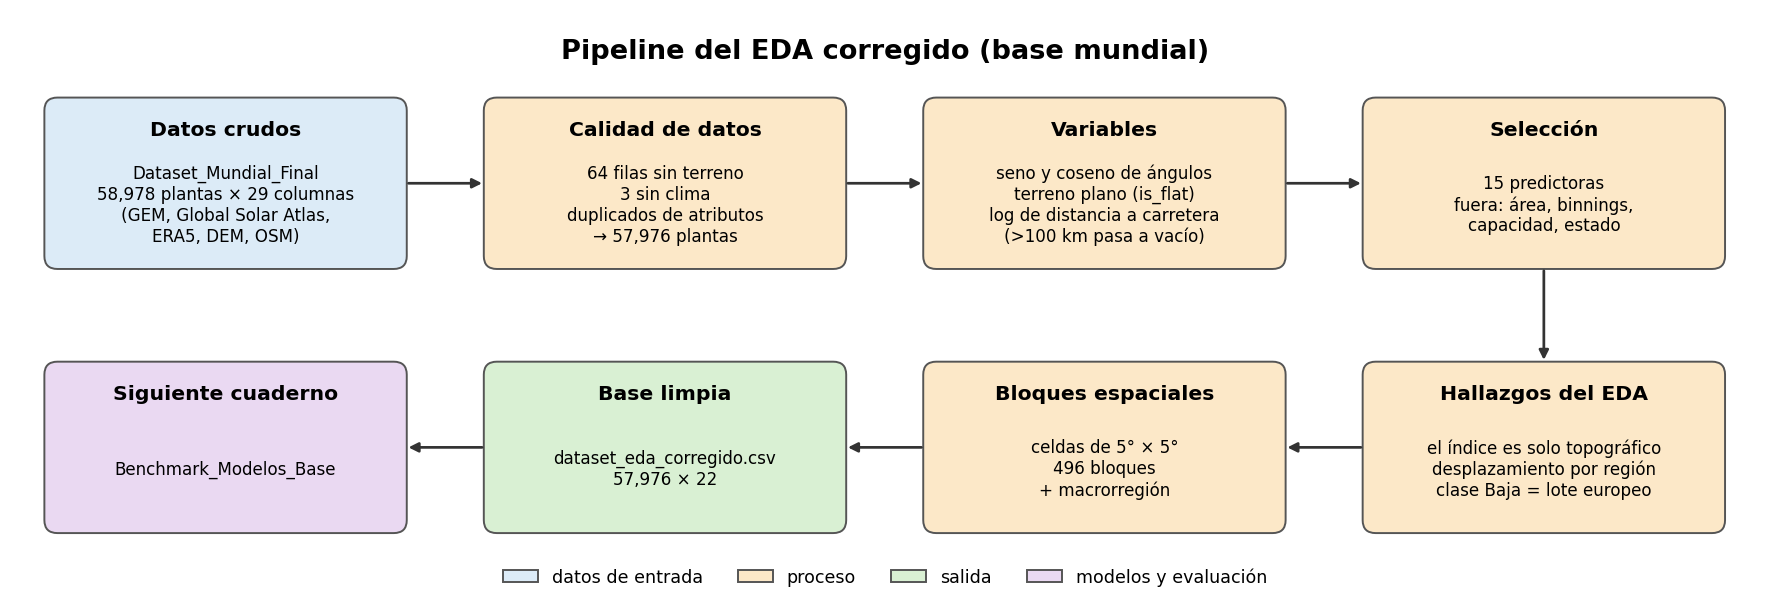
\includegraphics[width=\textwidth,height=0.82\textheight,keepaspectratio]{fig_pipeline_eda_mundial.png}
\end{frame}

\begin{frame}{Problemas de calidad de datos y decisiones}
  \centering
  \small
  \begin{tabularx}{\textwidth}{Xll}
    \toprule
    Problema & Cifra & Decisión \\
    \midrule
    Filas sin datos de terreno (todas clase Baja) & 64 & Eliminar \\
    Filas sin datos de clima & 3 & Eliminar \\
    Duplicados de atributos & 1,598 & Eliminar \\
    Orientación $-1$ en terreno plano & 1,105 & Seno, coseno e indicador \\
    Distancia a carretera imposible (hasta 2,296 km) & 65 & Vacío y logaritmo \\
    Área vacía o con densidades imposibles & 27.7\,\% & Excluir la variable \\
    Variables que son agrupaciones de otras & 5 & Excluir \\
    \bottomrule
  \end{tabularx}
  \vspace{0.5em}

  Resultado: \textbf{57,976 plantas y 15 predictoras}. Los ángulos van en seno y coseno porque 359° y 1° son vecinos (Fisher, 1993).
\end{frame}

\begin{frame}{El índice depende de la región}
  \centering
  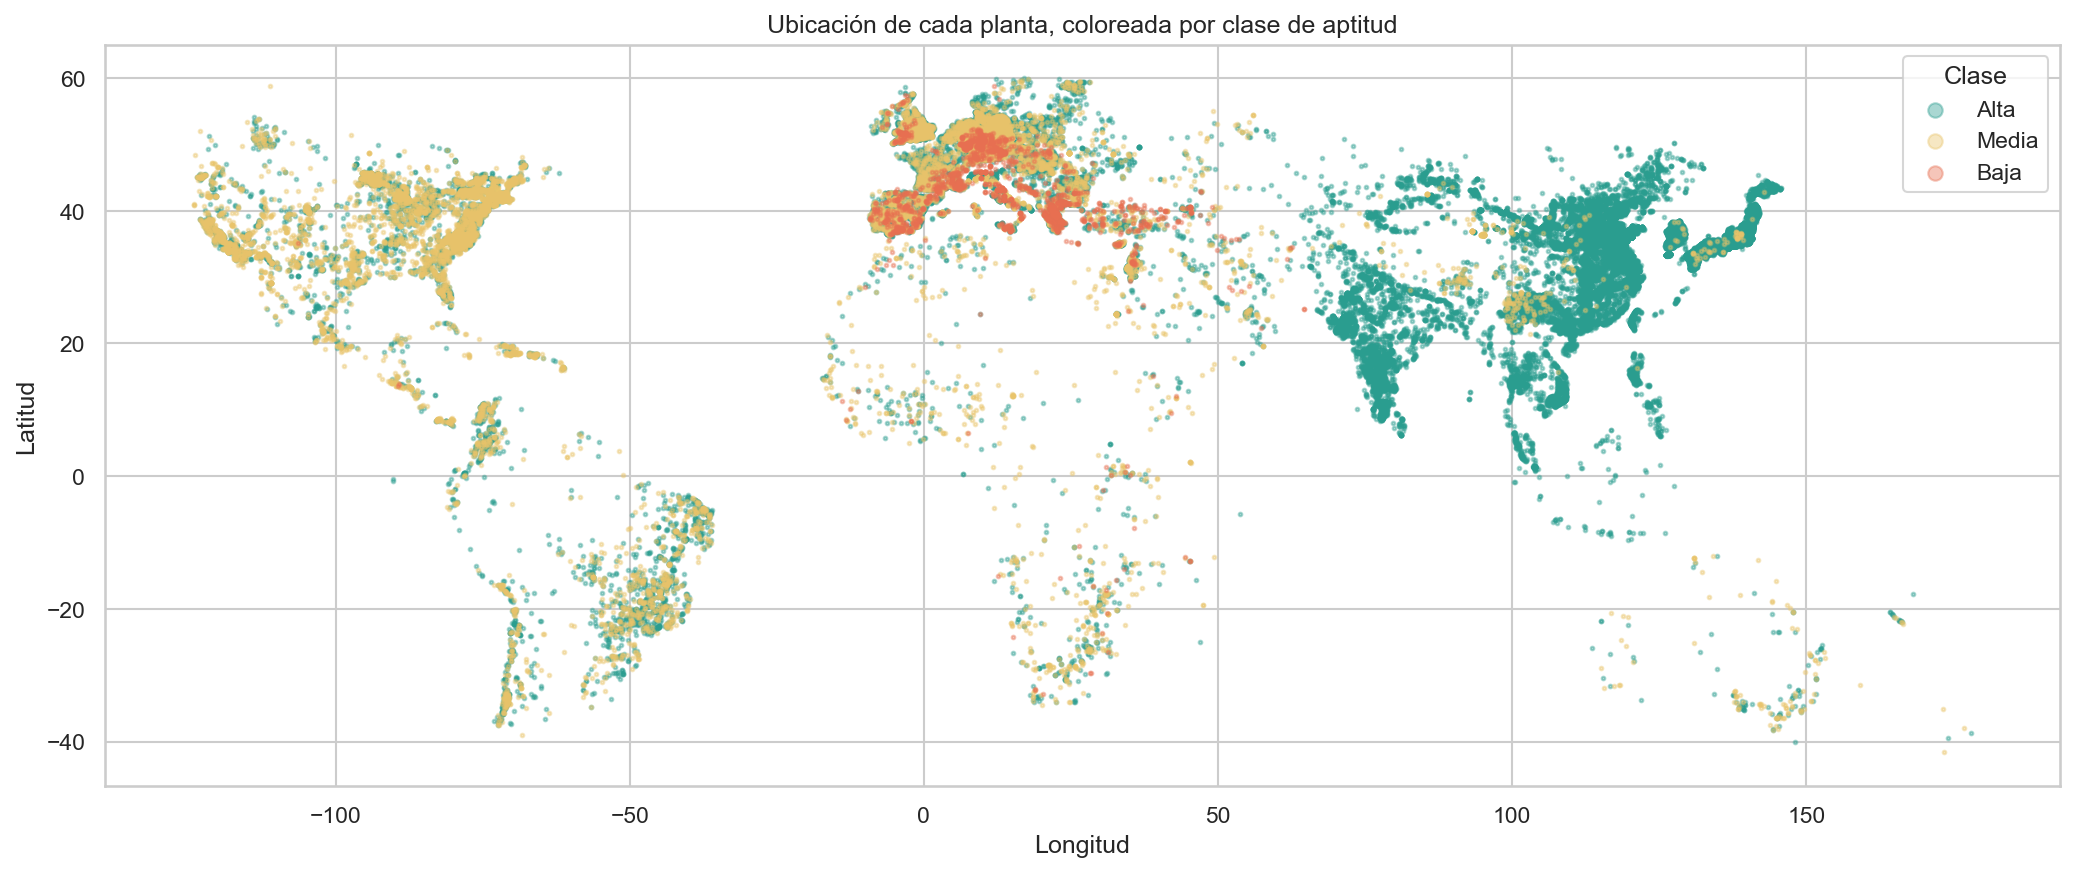
\includegraphics[width=\textwidth,height=0.62\textheight,keepaspectratio]{fig_mapa_clases_e3.png}
  \begin{itemize}
    \small
    \item Asia es casi toda Alta. La clase Baja aparece casi solo en Europa: el \alert{94.5\,\%} viene de un lote europeo añadido en la segunda versión del dataset.
  \end{itemize}
\end{frame}

\begin{frame}{Hallazgo central del EDA}
  \begin{columns}[T]
    \column{0.5\textwidth}
    \begin{itemize}
      \item Spearman del índice con la pendiente: \textbf{$-0.07$}. Con la longitud: \textbf{$+0.58$}.
      \item Modelo con solo terreno: \Rdos{} = 0.18.
      \item Añadiendo latitud y longitud: \Rdos{} = 0.91.
      \item Entrenando sin una macrorregión y prediciéndola: \Rdos{} negativo (de $-0.1$ a $-7.3$).
    \end{itemize}
    \column{0.48\textwidth}
    \begin{alertblock}{Conclusión}
      El índice depende sobre todo de la \textbf{región} y del \textbf{lote de procesamiento}. El terreno, que define su fórmula, pesa poco.
    \end{alertblock}
    \vspace{0.5em}
    \begin{block}{Implicación}
      La validación tiene que ser \textbf{espacial}: bloques de 5° $\times$ 5° (496 bloques).
    \end{block}
  \end{columns}
\end{frame}

\begin{frame}{Base nueva: generación real en Colombia}
  \centering
  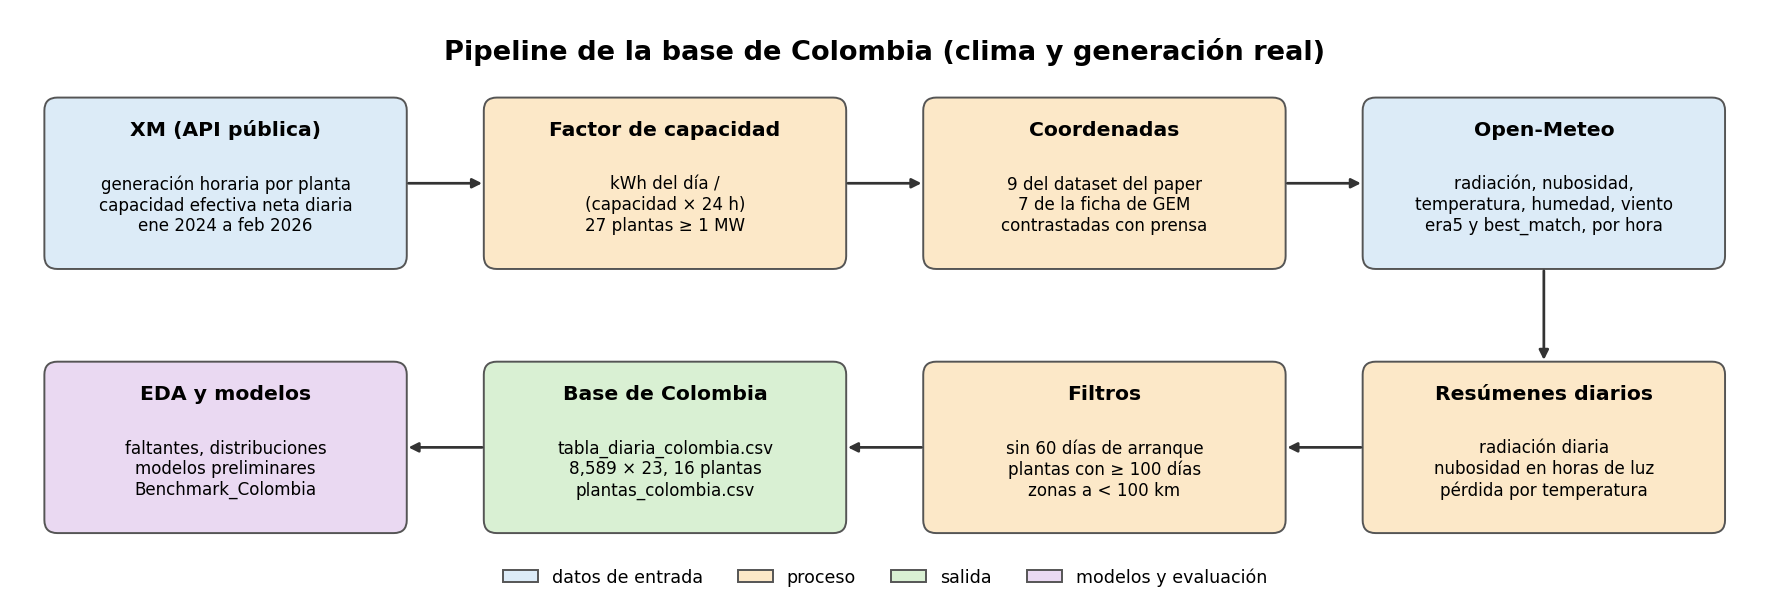
\includegraphics[width=\textwidth,height=0.80\textheight,keepaspectratio]{fig_pipeline_clima.png}
\end{frame}

\begin{frame}{Cómo se construyó la base de Colombia}
  \begin{itemize}
    \item \textbf{XM}: generación horaria y capacidad diaria, enero 2024 a febrero 2026.
    \item \textbf{Factor de capacidad} (FC) = energía del día / (capacidad $\times$ 24 h). Es la variable que predecimos.
    \item \textbf{Coordenadas}: XM no las publica. 9 plantas del dataset y 7 de la ficha de GEM, cada una verificada con prensa o el desarrollador.
          \\ Descartadas: Palmira II (ubicación sin confirmar) y Shangri-La (coordenadas de GEM contradicen su ficha).
    \item \textbf{Clima} por hora de Open-Meteo, dos productos: ERA5 y \texttt{best\_match}.
    \item \textbf{Filtros} que no miran la variable a predecir: sin 60 días de arranque, plantas con al menos 100 días.
    \item Resultado: \alert{8,589 días planta, 16 plantas, 6 zonas, sin valores vacíos}.
  \end{itemize}
\end{frame}

\begin{frame}{EDA de la base de Colombia}
  \centering
  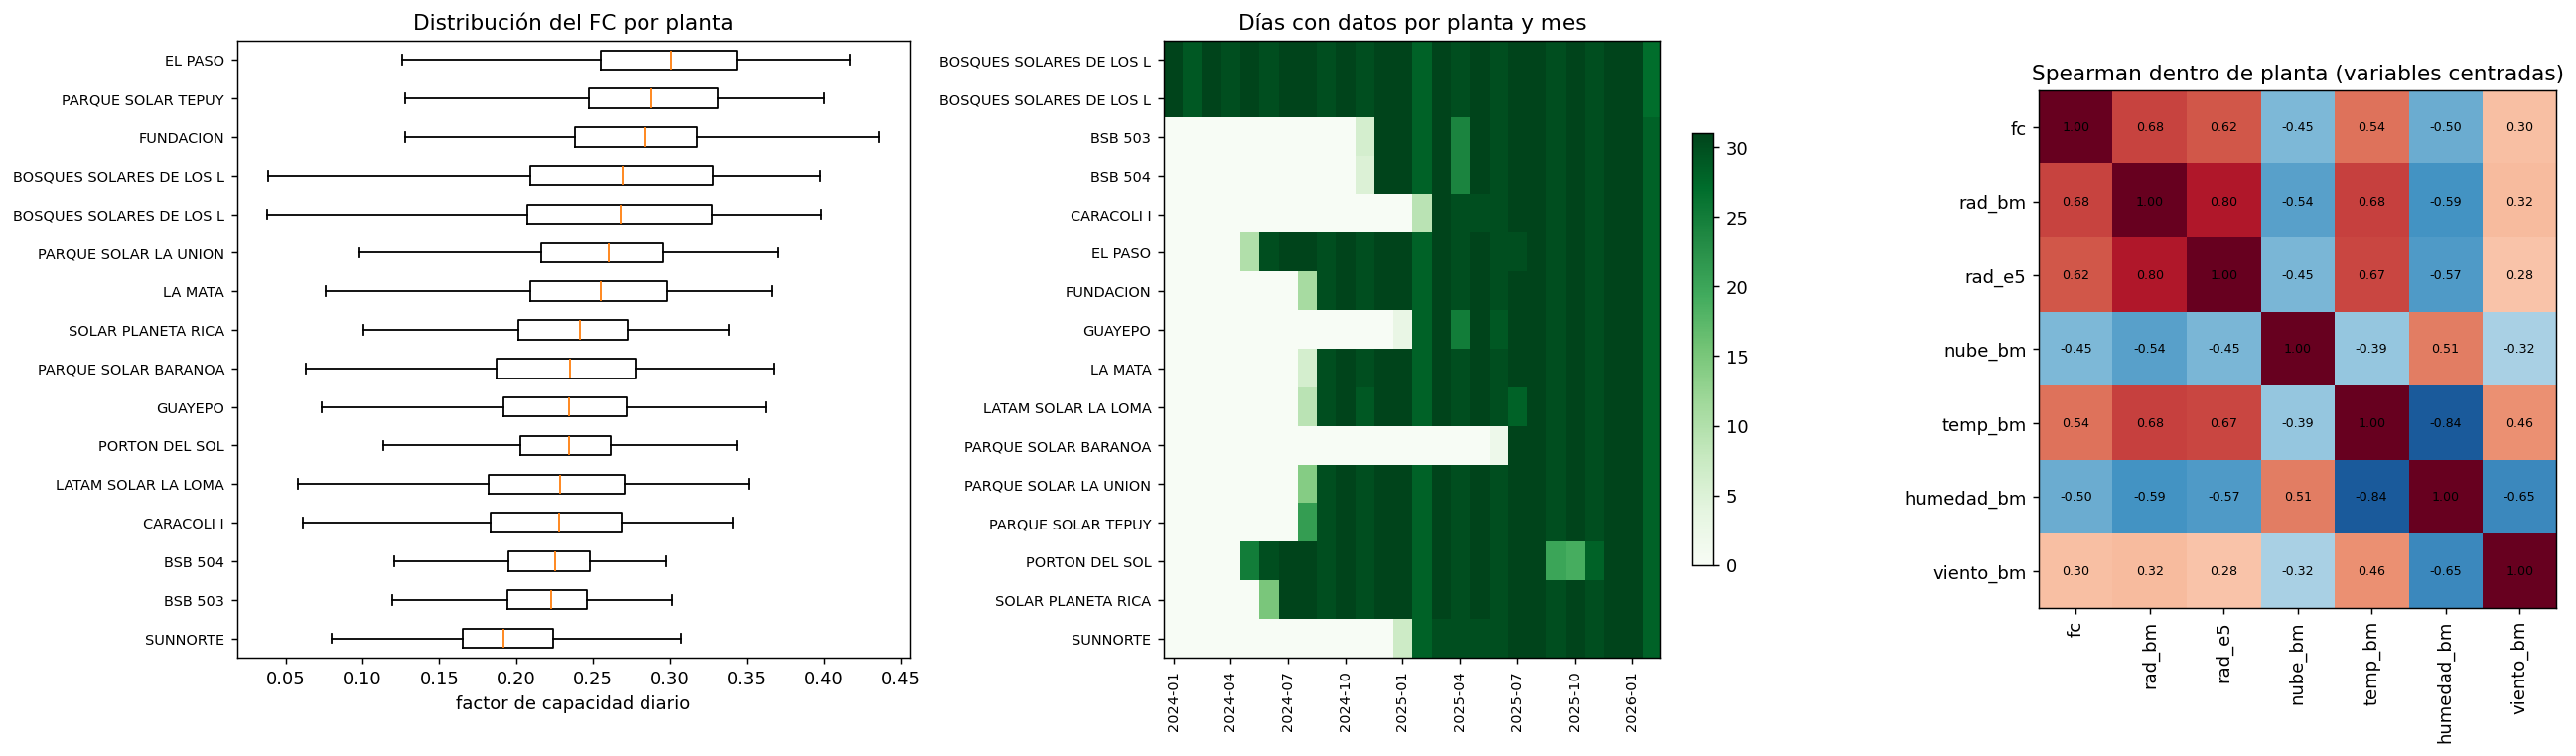
\includegraphics[width=\textwidth,height=0.62\textheight,keepaspectratio]{fig_eda_base_colombia.png}
  \begin{itemize}
    \small
    \item El 84\,\% de la variación del FC es de un día a otro dentro de cada planta. El 16\,\% es entre plantas (tecnología: pendiente).
    \item Radiación, nubosidad, temperatura y humedad están muy correlacionadas entre sí.
  \end{itemize}
\end{frame}

\begin{frame}{La radiación explica el día a día}
  \centering
  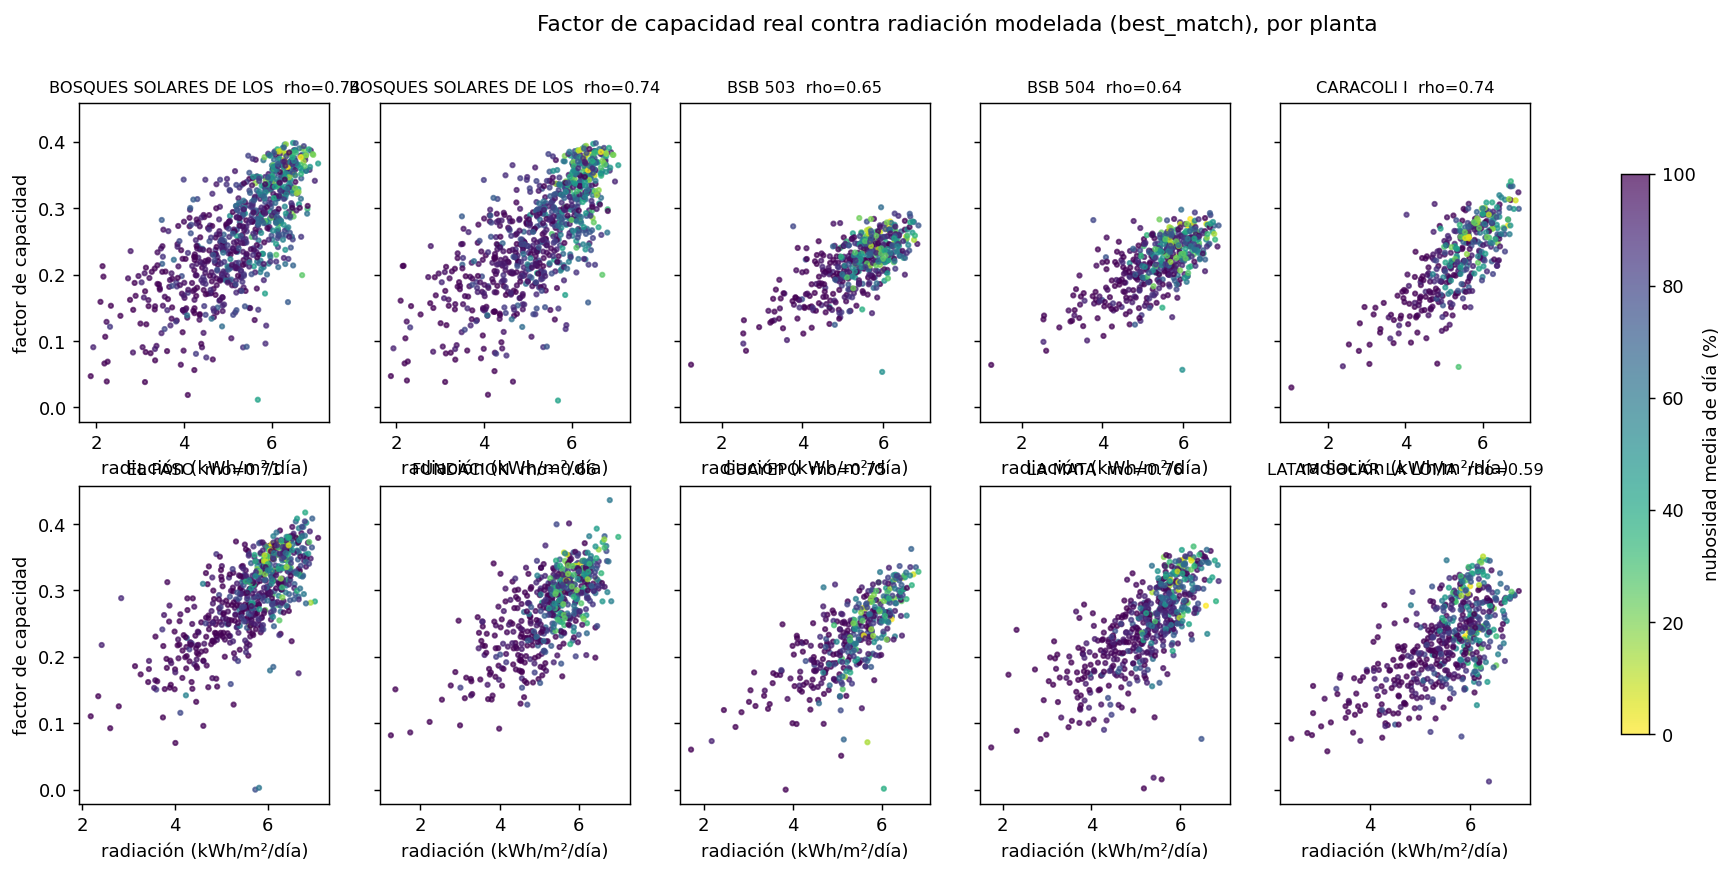
\includegraphics[width=\textwidth,height=0.66\textheight,keepaspectratio]{fig_fc_vs_radiacion.png}
  \begin{itemize}
    \small
    \item Cada kWh/m² de radiación diaria suma unos \textbf{4.7 puntos de FC}, casi la proporción física simple.
    \item La radiación de \texttt{best\_match} explica más que la de ERA5 en 13 de 16 plantas.
  \end{itemize}
\end{frame}

% =====================================================================
\section{Parte 2. Modelos y evaluación}
% =====================================================================

\begin{frame}{Diseño experimental: la partición va primero}
  \begin{columns}[T]
    \column{0.52\textwidth}
    \begin{itemize}
      \item \textbf{Base mundial}: 5 folds por bloques de 5° $\times$ 5°. Un bloque entero va a entrenamiento o a prueba (Roberts et al., 2017).
      \item \textbf{Colombia}: se deja fuera una zona completa y se entrena con el pasado de cada planta para probar en su futuro.
      \item Imputación, escalado y calibración van dentro de un \texttt{Pipeline}: se ajustan solo con entrenamiento (Kaufman et al., 2012).
    \end{itemize}
    \column{0.46\textwidth}
    \begin{block}{nested CV}
      inner loop: elige hiperparámetros, también por bloques o zonas. \\[0.3em]
      outer loop: solo mide. \\[0.3em]
      Así el resultado no sale inflado por haber elegido mirando la prueba (Varma y Simon, 2006; Cawley y Talbot, 2010).
    \end{block}
  \end{columns}
\end{frame}

\begin{frame}{Pipeline de evaluación}
  \centering
  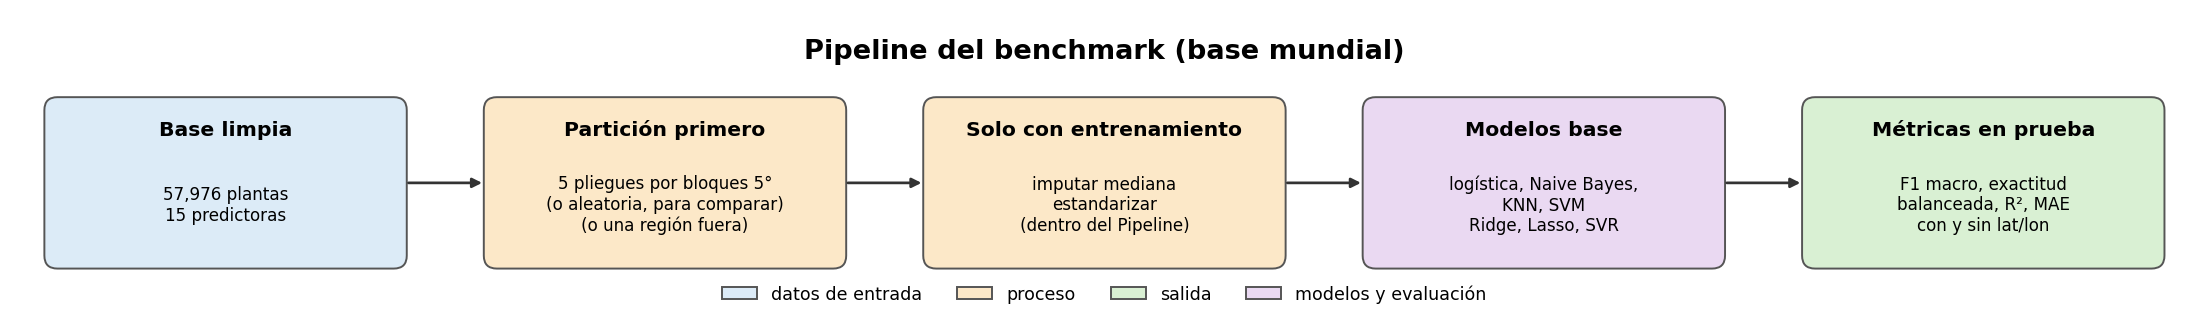
\includegraphics[width=\textwidth,height=0.42\textheight,keepaspectratio]{fig_pipeline_benchmark_mundial.png}\\[0.4em]
  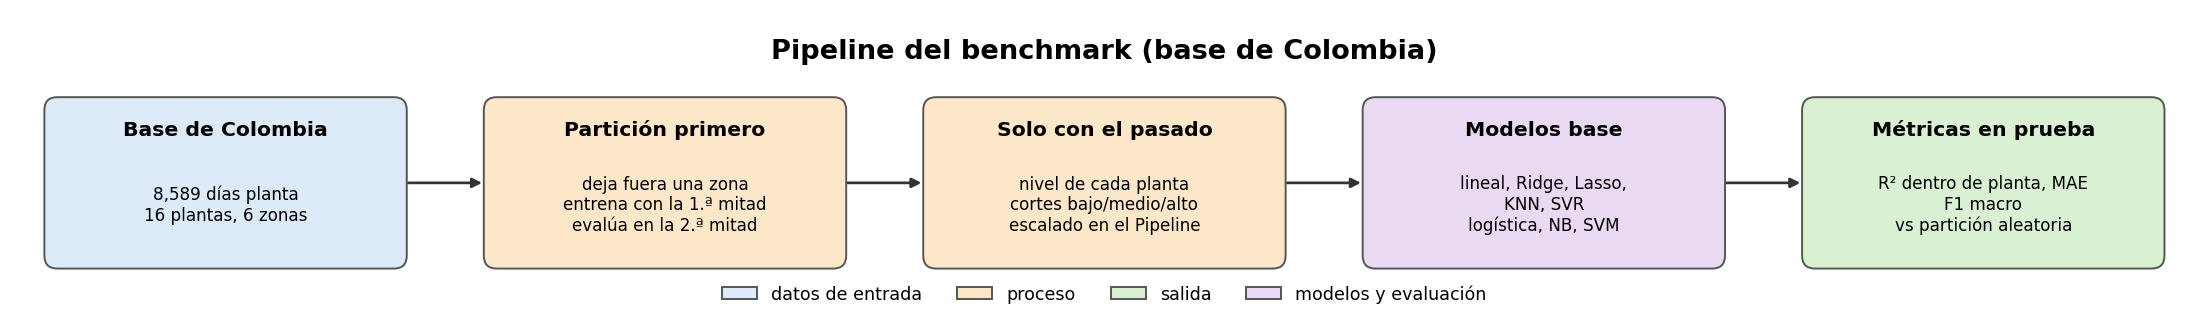
\includegraphics[width=\textwidth,height=0.42\textheight,keepaspectratio]{fig_pipeline_benchmark_colombia.png}
\end{frame}

\begin{frame}{Modelos y métricas}
  \begin{columns}[T]
    \column{0.47\textwidth}
    \textbf{Modelos base del curso}
    \begin{itemize}
      \item Clasificación: regresión logística (normal y balanceada), Naive Bayes, KNN, SVM lineal y SVM RBF.
      \item Regresión: Ridge, Lasso, KNN, SVR lineal y SVR RBF.
      \item Referencia: clase mayoritaria, media o nivel de la planta.
      \item Hiperparámetros con búsqueda en grilla, escala logarítmica para C y alpha (Bergstra y Bengio, 2012).
    \end{itemize}
    \column{0.5\textwidth}
    \textbf{Métricas}
    \begin{itemize}
      \item \textbf{F1 macro}: principal, porque la clase Baja es el 3\,\% (He y Garcia, 2009).
      \item \textbf{AUC} uno contra el resto: calidad de las probabilidades sin umbral (Fawcett, 2006).
      \item \textbf{Kappa ponderado}: las clases tienen orden (Cohen, 1968).
      \item Exactitud balanceada, precisión, recall, F1 de Baja.
      \item Regresión: \Rdos{}, RMSE y MAE.
    \end{itemize}
  \end{columns}
\end{frame}

\begin{frame}{Resultados: comparativa de todos los modelos ajustados}
  \centering
  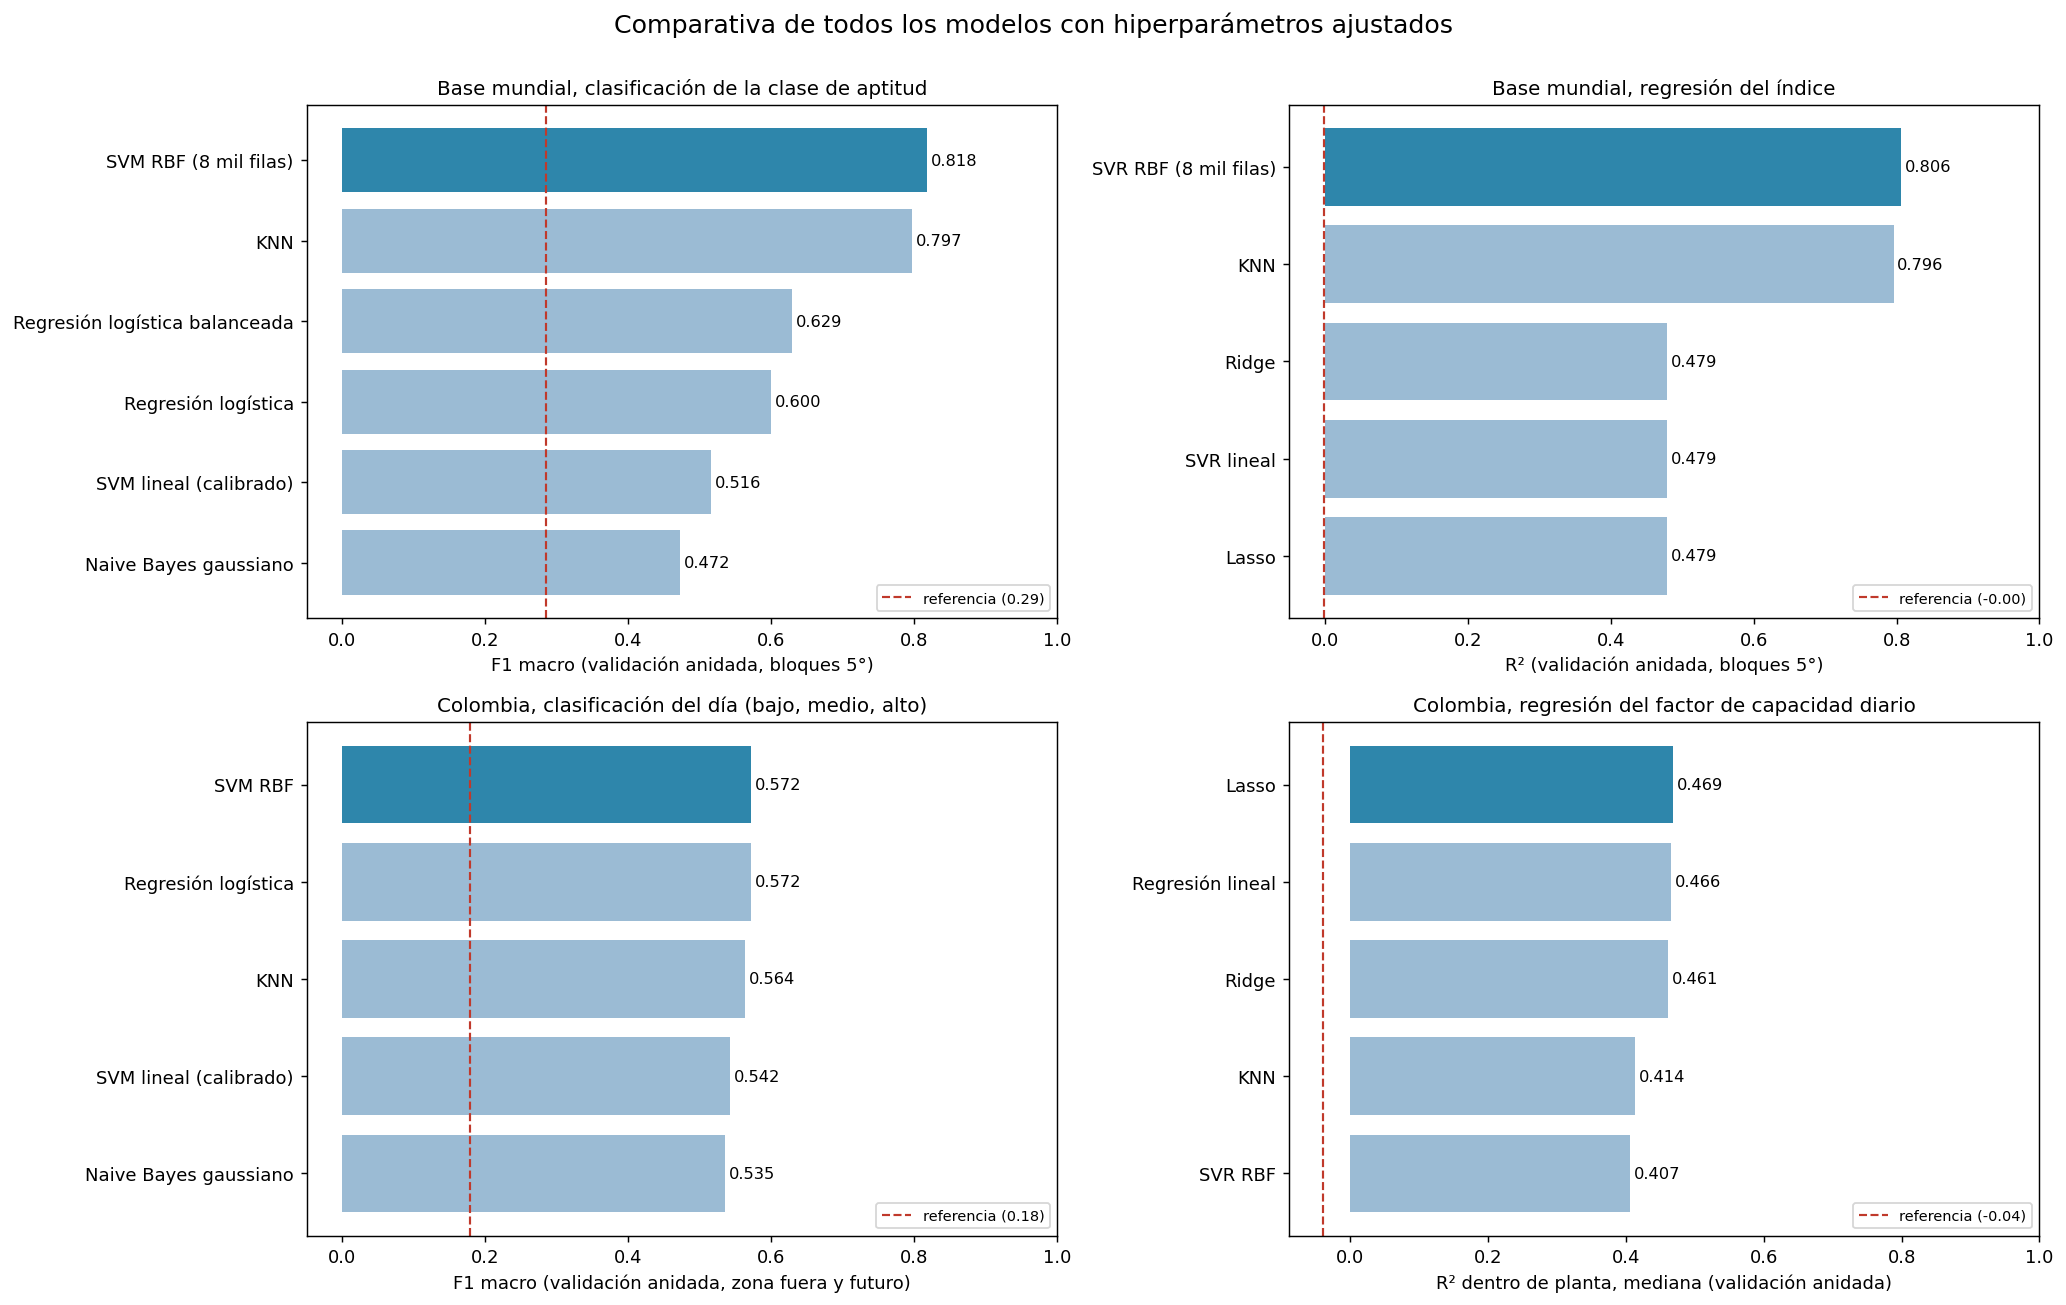
\includegraphics[width=\textwidth,height=0.86\textheight,keepaspectratio]{fig_resumen_comparativa.png}
\end{frame}

\begin{frame}{Base mundial: clasificación (ajustada, bloques 5°)}
  \centering
  \small
  \begin{tabular}{lccccc}
    \toprule
    Modelo & F1 macro & Exact. bal. & AUC & Kappa & F1 Baja \\
    \midrule
    \textbf{SVM RBF} & \textbf{0.818} & 0.793 & \textbf{0.960} & \textbf{0.775} & \textbf{0.744} \\
    KNN & 0.797 & 0.767 & 0.925 & 0.753 & 0.694 \\
    Logística balanceada & 0.629 & \textbf{0.798} & 0.873 & 0.482 & 0.506 \\
    Logística & 0.600 & 0.560 & 0.865 & 0.368 & 0.525 \\
    SVM lineal & 0.516 & 0.479 & 0.874 & 0.246 & 0.358 \\
    Naive Bayes & 0.472 & 0.674 & 0.835 & 0.289 & 0.208 \\
    Referencia & 0.285 & 0.333 & 0.500 & 0.000 & 0.000 \\
    \bottomrule
  \end{tabular}
  \vspace{0.6em}

  Regresión del índice: \textbf{SVR RBF \Rdos{} = 0.806}, KNN 0.796, Ridge y Lasso 0.479, referencia $-0.002$.
\end{frame}

\begin{frame}{Base mundial: ROC y matriz de confusión}
  \centering
  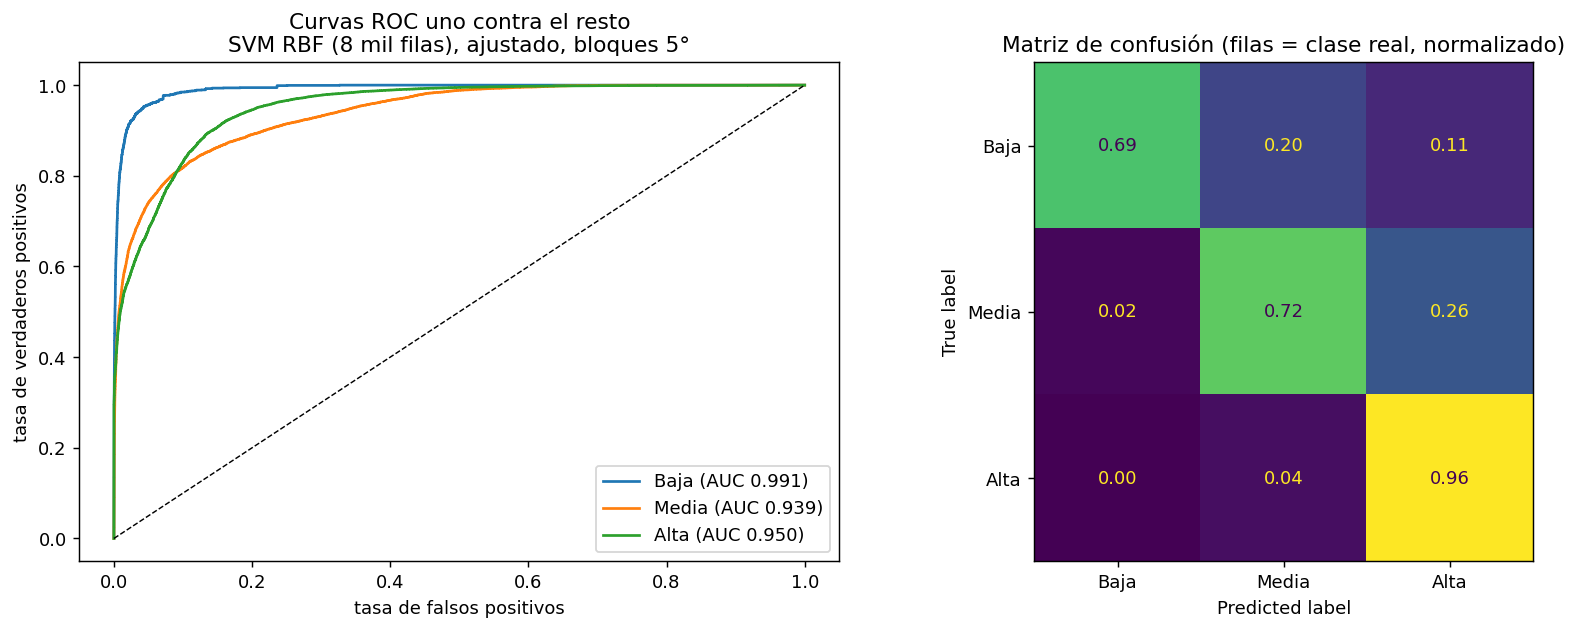
\includegraphics[width=\textwidth,height=0.84\textheight,keepaspectratio]{fig_benchmark_roc_confusion.png}
\end{frame}

\begin{frame}{¿Qué aprendieron los modelos?}
  \centering
  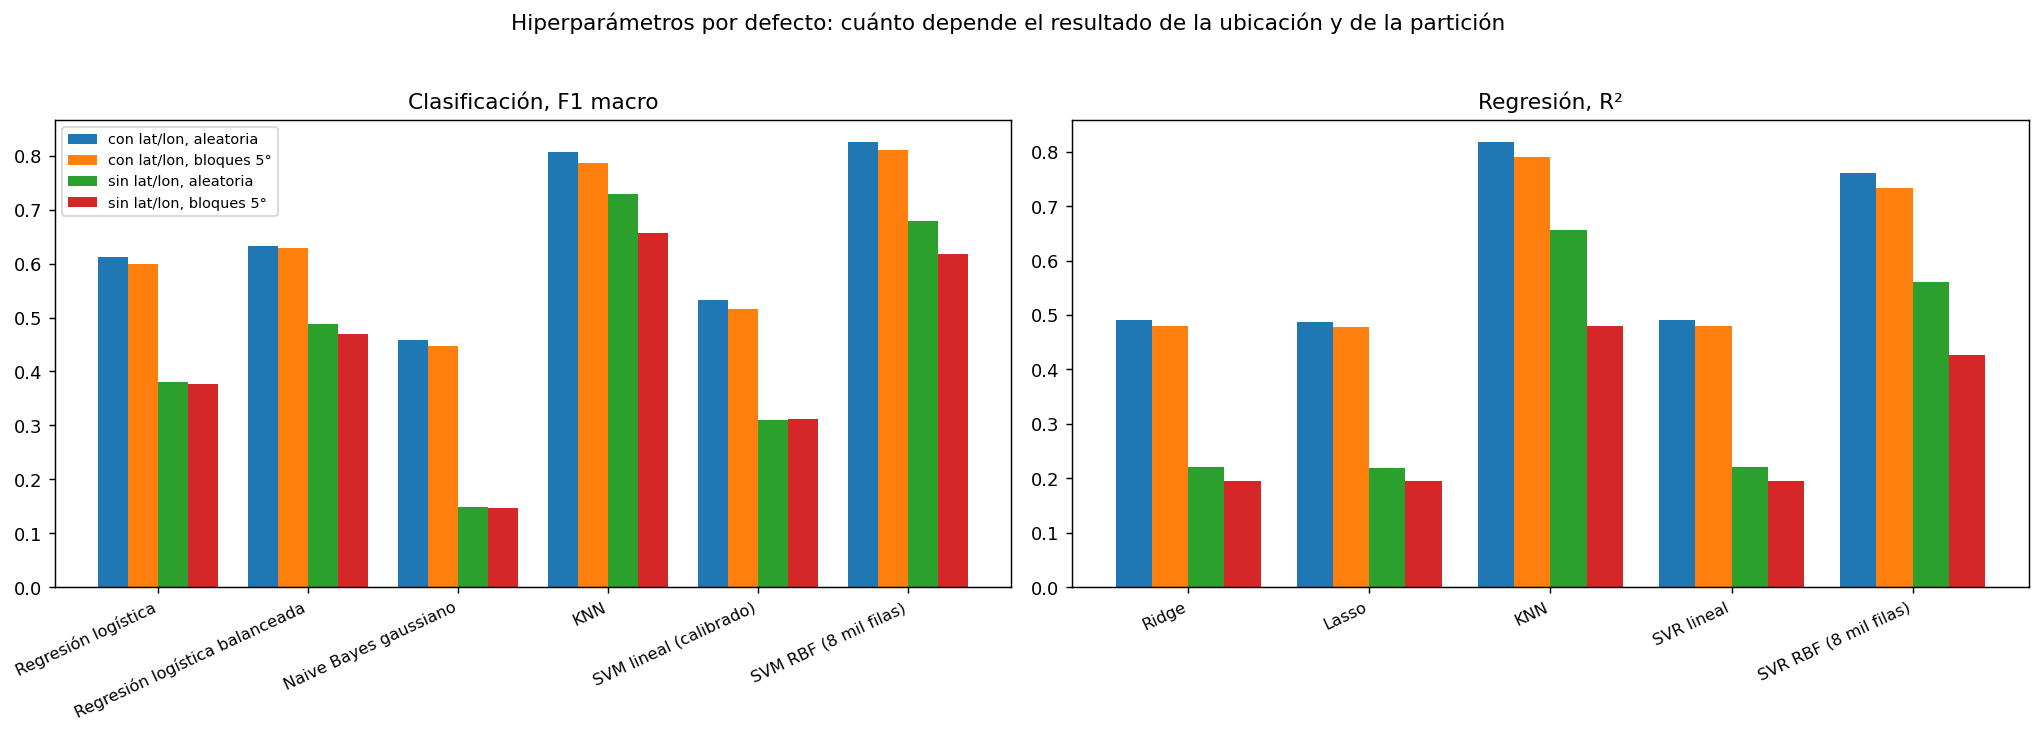
\includegraphics[width=\textwidth,height=0.55\textheight,keepaspectratio]{fig_benchmark_modelos.png}
  \begin{itemize}
    \small
    \item Sin latitud y longitud, KNN cae de \Rdos{} 0.79 a 0.48: aprende \alert{dónde} está la planta.
    \item La partición aleatoria da resultados más altos que los bloques.
    \item Dejando un continente fuera, \alert{todos} dan \Rdos{} negativo, incluida la referencia.
  \end{itemize}
\end{frame}

\begin{frame}{Colombia: resultados (ajustados, Leave-Region-Out y futuro)}
  \begin{columns}[T]
    \column{0.48\textwidth}
    \textbf{Regresión del FC diario}\\[0.3em]
    \small
    \begin{tabular}{lcc}
      \toprule
      Modelo & \Rdos{} planta & MAE rel. \\
      \midrule
      \textbf{Lasso} & \textbf{0.469} & \textbf{0.140} \\
      Lineal & 0.466 & 0.141 \\
      Ridge & 0.461 & 0.141 \\
      KNN & 0.414 & 0.147 \\
      SVR RBF & 0.407 & 0.144 \\
      Referencia & $-0.039$ & 0.196 \\
      \bottomrule
    \end{tabular}
    \column{0.5\textwidth}
    \textbf{Día bajo, medio o alto}\\[0.3em]
    \small
    \begin{tabular}{lccc}
      \toprule
      Modelo & F1 & AUC & Kappa \\
      \midrule
      \textbf{Logística} & \textbf{0.572} & \textbf{0.765} & \textbf{0.575} \\
      SVM RBF & 0.572 & 0.759 & 0.568 \\
      KNN & 0.564 & 0.753 & 0.561 \\
      SVM lineal & 0.542 & 0.751 & 0.553 \\
      Naive Bayes & 0.535 & 0.737 & 0.508 \\
      Referencia & 0.178 & 0.500 & 0.000 \\
      \bottomrule
    \end{tabular}
  \end{columns}
  \vspace{0.6em}
  \begin{itemize}
    \small
    \item Aquí ganan los \textbf{lineales}: la energía es casi proporcional a la radiación. El error baja del 20\,\% al 14\,\% del FC medio.
  \end{itemize}
\end{frame}

\begin{frame}{Colombia: contrastes}
  \centering
  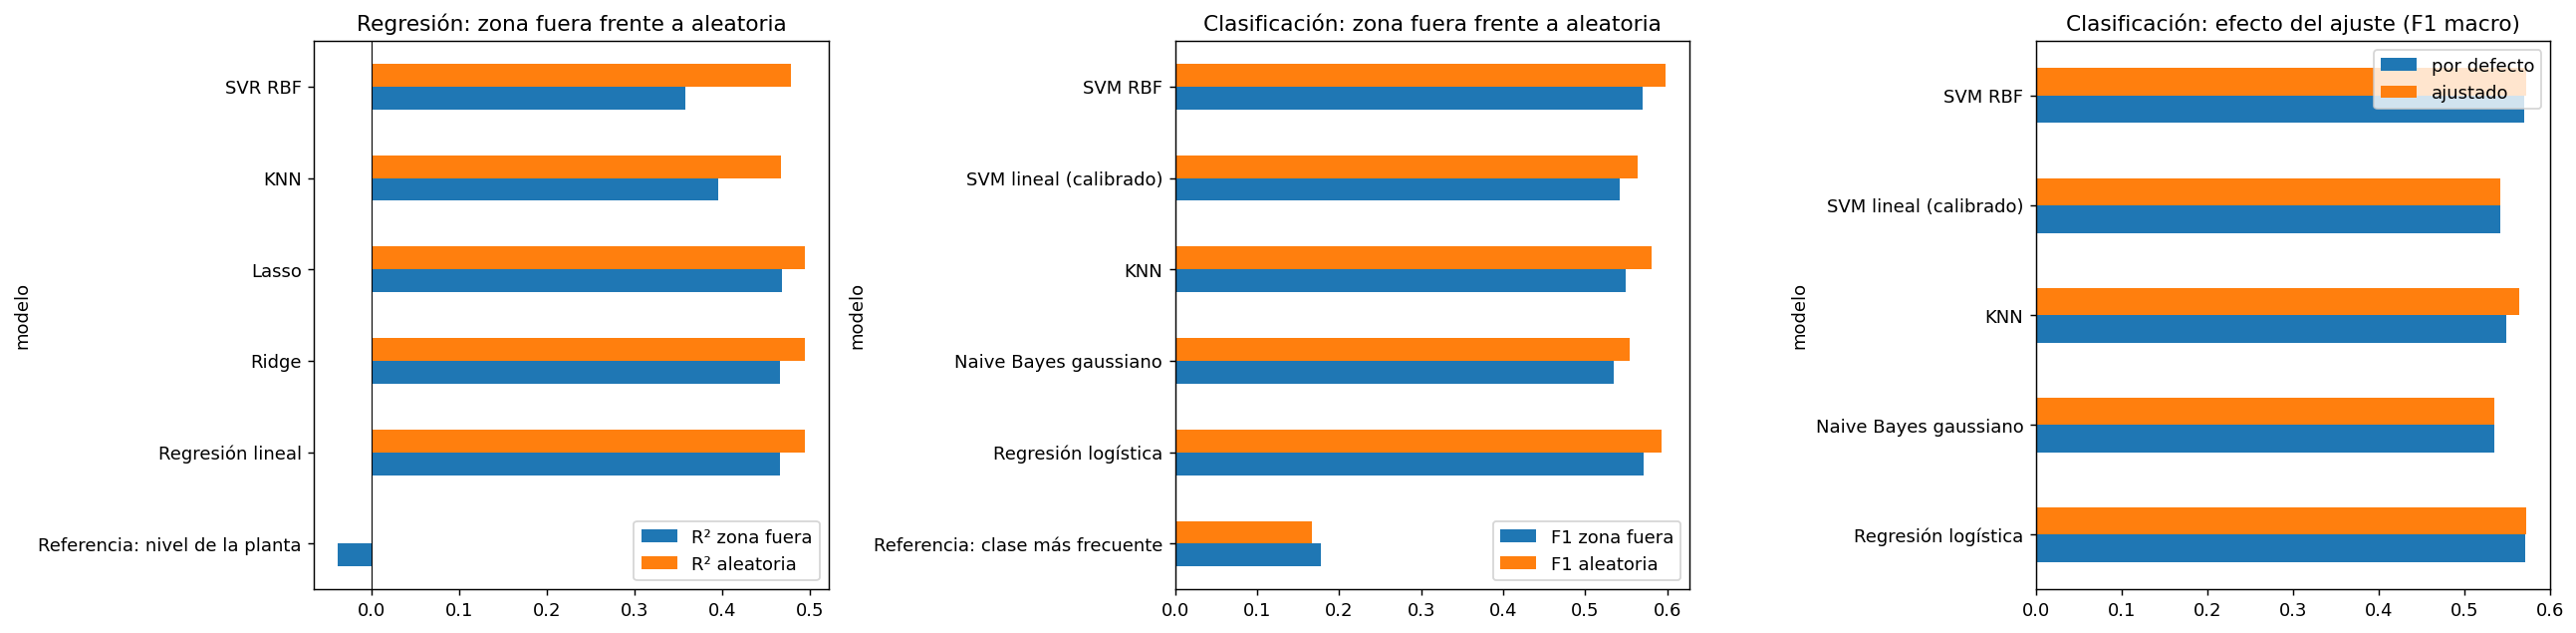
\includegraphics[width=\textwidth,height=0.55\textheight,keepaspectratio]{fig_benchmark_colombia.png}
  \begin{itemize}
    \small
    \item Con partición aleatoria el SVR sube de \Rdos{} 0.36 a 0.48: el resultado se infla.
    \item Con solo la radiación, el SVR sube de 0.36 a 0.49: las demás variables agregan ruido.
    \item El ajuste eligió siempre la opción más suave (KNN con 101 vecinos, SVR con C = 0.1).
  \end{itemize}
\end{frame}

\begin{frame}{Interpretación: ¿por qué unos modelos quedan bajos?}
  \begin{columns}[T]
    \column{0.49\textwidth}
    \textbf{Base mundial}
    \begin{itemize}
      \small
      \item Un modelo lineal ajusta un solo plano para todo el mundo; el índice cambia de nivel por región (no estacionariedad espacial, Brunsdon et al., 1996).
      \item KNN y SVM con kernel ajustan vecindarios locales.
      \item Lasso no mejora: con 15 variables y 58 mil filas, la regularización casi no cambia el ajuste.
      \item Naive Bayes supone independencia y normalidad.
    \end{itemize}
    \column{0.49\textwidth}
    \textbf{Colombia}
    \begin{itemize}
      \small
      \item La física es casi lineal y hay solo 6 zonas: los modelos flexibles sobreajustan.
      \item El techo ($\approx 0.5$) está en los datos: radiación modelada, promedios diarios y tecnología sin medir.
    \end{itemize}
  \end{columns}
\end{frame}

\begin{frame}{¿Cómo se podría mejorar?}
  \begin{columns}[T]
    \column{0.49\textwidth}
    \textbf{Base mundial}
    \begin{itemize}
      \small
      \item Bosques aleatorios (Breiman, 2001) y XGBoost (Chen y Guestrin, 2016).
      \item Modelos espaciales: bosque aleatorio espacial (Hengl et al., 2018) o regresión geográficamente ponderada.
      \item Stacking de varios modelos (Wolpert, 1992).
      \item Un puntaje más alto no haría que el índice mida aptitud. Conviene delimitar el área de aplicabilidad (Meyer y Pebesma, 2021).
    \end{itemize}
    \column{0.49\textwidth}
    \textbf{Colombia}
    \begin{itemize}
      \small
      \item Modelo híbrido físico + ML con pvlib (Holmgren et al., 2018; Antonanzas et al., 2016).
      \item Radiación satelital o medida en lugar de reanálisis.
      \item Efectos mixtos por planta (Bates et al., 2015; Hajjem et al., 2014).
      \item Datos horarios e índice de claridad.
      \item Completar la tecnología de cada planta.
    \end{itemize}
  \end{columns}
\end{frame}

\begin{frame}{Entregable 2: Experimento combinatorio (140 combinaciones)}
  \begin{columns}[T]
    \column{0.48\textwidth}
    \textbf{Estructura combinatoria}
    \begin{itemize}
      \small
      \item \textbf{Clasificación:} 7 modelos $\times$ 4 balanceos $\times$ 4 optimizadores = 112 combinaciones.
      \item \textbf{Regresión:} 7 modelos $\times$ 4 optimizadores = 28 combinaciones.
      \item \textbf{Total:} 140 combinaciones en 5 outer folds y 3 internos (700 modelos).
      \item Balanceos: ninguno, SMOTE, ADASYN, \texttt{class\_weight}.
    \end{itemize}
    \column{0.48\textwidth}
    \textbf{Optimizadores comparados}
    \begin{itemize}
      \small
      \item \textbf{Grid Search:} barrido factorial en malla discreta.
      \item \textbf{Random Search:} muestreo uniforme estocástico.
      \item \textbf{Bayesiano (Optuna):} estimador TPE kernelizado.
      \item \textbf{Genético (DEAP):} torneo, cruce y mutación.
      \item Presupuesto uniforme: $B = 30$ evaluaciones/fold.
    \end{itemize}
  \end{columns}
\end{frame}

\begin{frame}{Comparación de optimizadores: Desempeño anytime}
  \centering
  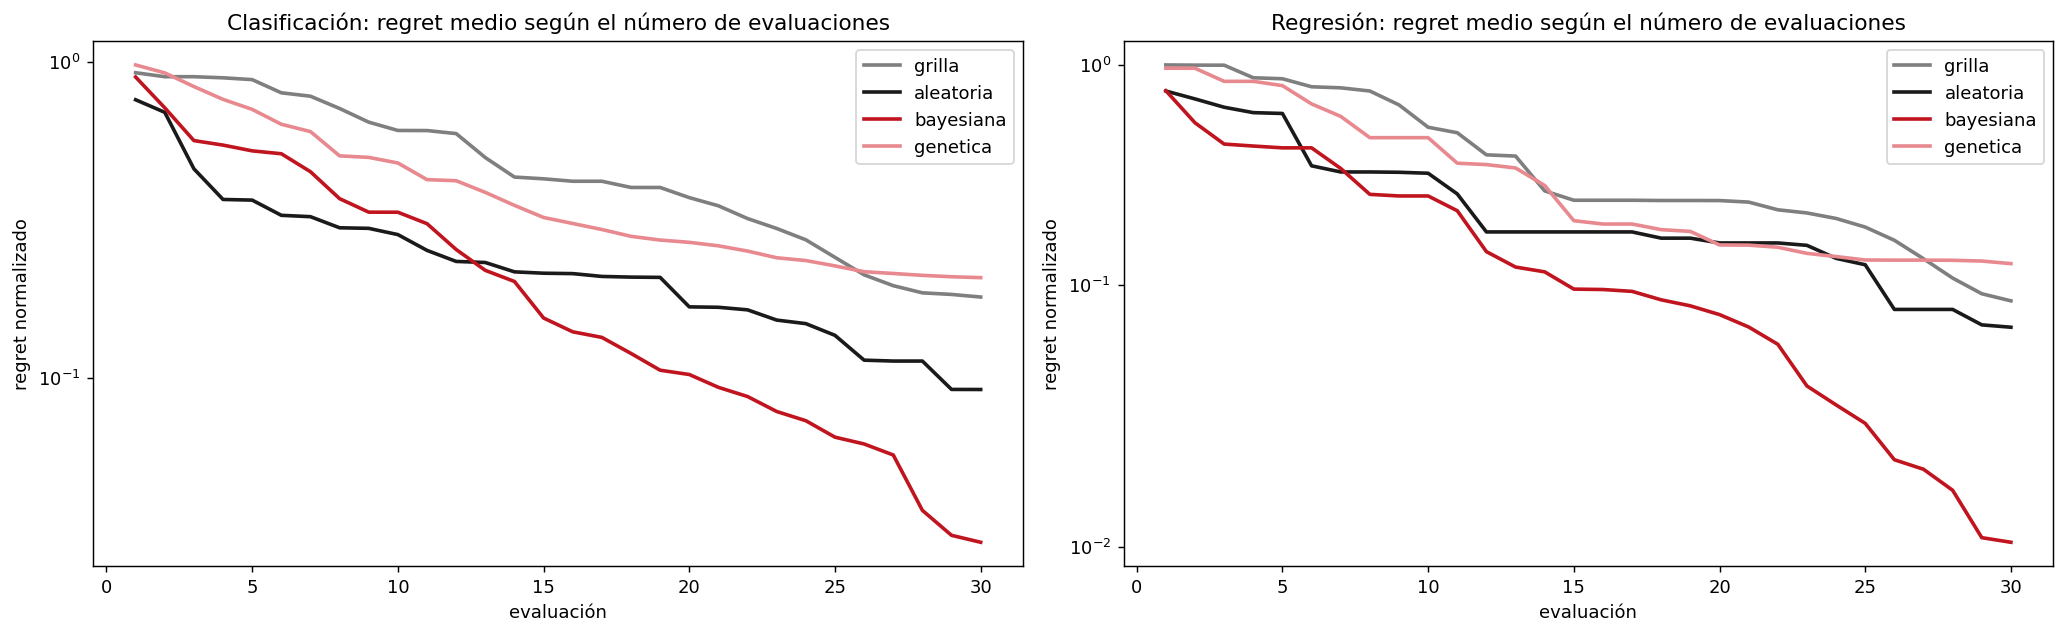
\includegraphics[width=\textwidth,height=0.68\textheight,keepaspectratio]{fig_exp_anytime.png}
  \begin{itemize}
    \small
    \item \textbf{Optuna (TPE)} alcanza el 95\,\% del óptimo hacia la iteración 15; explora cuencas promisorias con mayor eficiencia.
    \item El algoritmo genético sufre pérdida prematura de diversidad alélica con presupuesto acotado ($N=10$).
    \item Random Search provee una línea base competitiva en espacios con pocas dimensiones activas.
  \end{itemize}
\end{frame}

\begin{frame}{Validación estadística formal: Nemenyi y diferencias críticas}
  \centering
  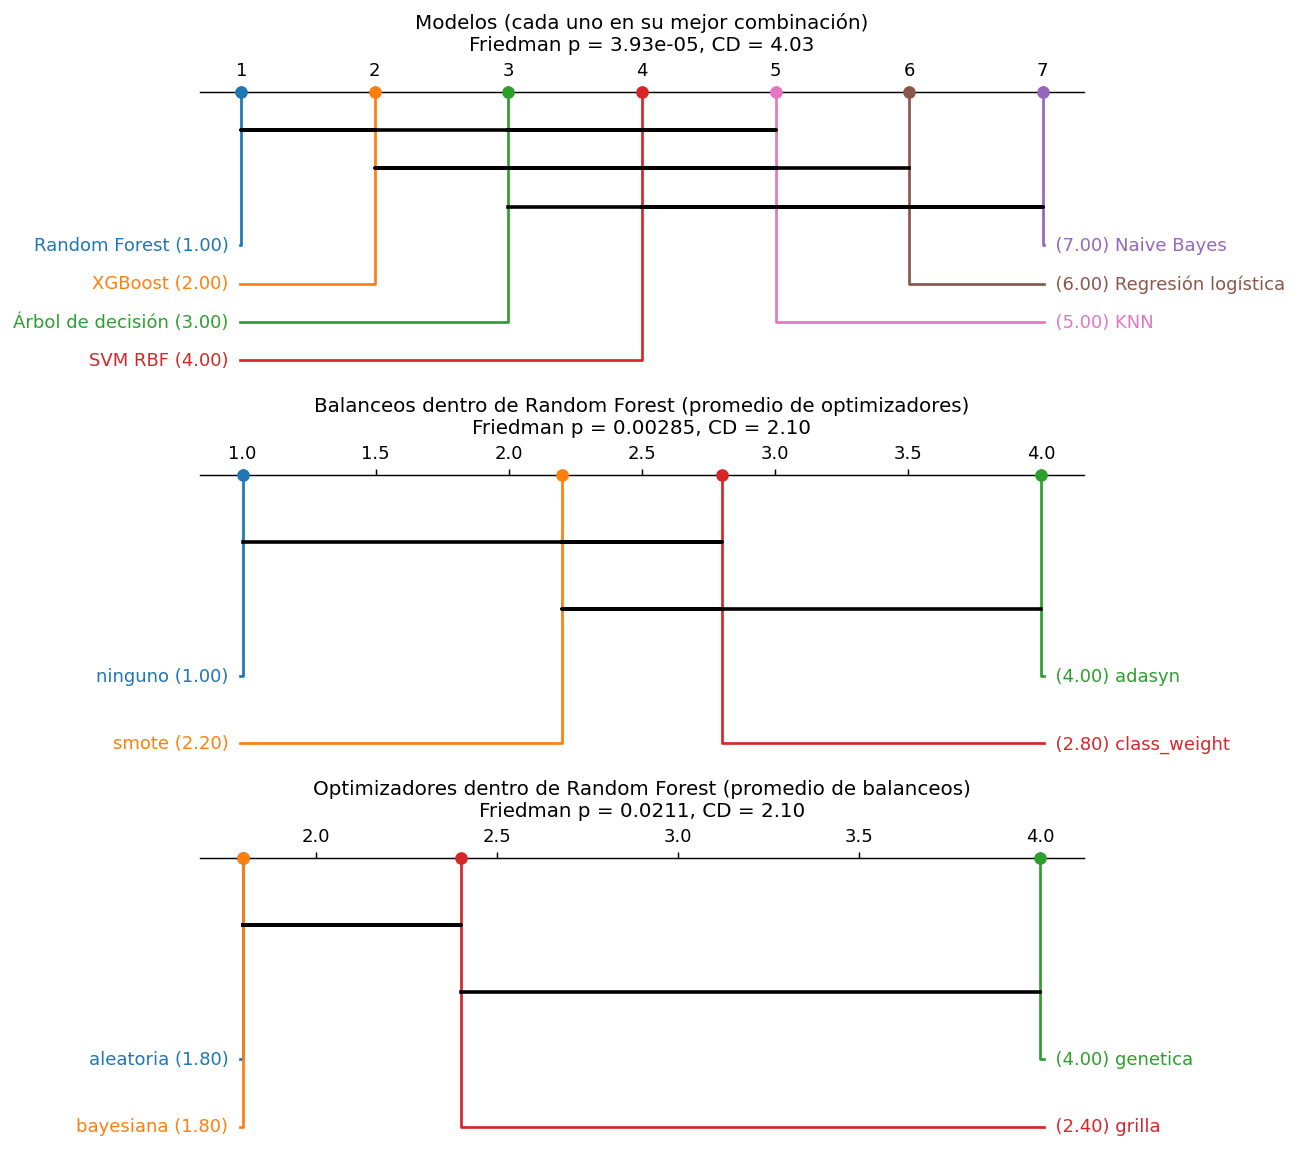
\includegraphics[width=\textwidth,height=0.66\textheight,keepaspectratio]{fig_exp_cd.png}
  \begin{itemize}
    \small
    \item Test de Friedman: $\chi^2 = 527.17$ ($p = 8.98 \times 10^{-57}$), confirmando diferencias entre algoritmos.
    \item \textbf{Random Forest y XGBoost} forman el cluster estadísticamente superior (DeLong $p = 0.254$).
    \item El Model Confidence Set (MCS al 90\,\%) descarta árboles simples, KNN, SVM y modelos lineales.
  \end{itemize}
\end{frame}

\begin{frame}{Los resultados en tres números}
  \vspace{1.5em}
  \centering
  \cifra{0.90}{F1 macro de los ensambles líderes (Random Forest y XGBoost) en validación espacial}\hfill
  \cifra{15}{iteraciones promedio de Optuna para alcanzar el 95\,\% del puntaje óptimo}\hfill
  \cifra{0.47}{\Rdos{} del clima sobre la producción diaria real en Colombia}

  \vspace{2em}
  \small Un buen puntaje dentro de una región reproduce divisiones del procesamiento, no aptitud física del terreno.
\end{frame}

\begin{frame}{Conclusiones}
  \begin{enumerate}
    \item El índice del dataset mide terreno, región y lote de procesamiento; no se predice desde el clima ni se transfiere entre continentes.
    \item En la base mundial, Random Forest ($F1 = 0.897, R^2 = 0.902$) y XGBoost ($F1 = 0.896, R^2 = 0.899$) dominan de forma indistinguible ($p_{DM} = 0.184$).
    \item La optimización bayesiana (Optuna) superó sistemáticamente a Grid y Genético en velocidad de convergencia.
    \item En la base real de Colombia, el clima explica el 47\,\% de la variación diaria (\Rdos{} $\approx$ 0.47) y los modelos lineales resultan suficientes.
  \end{enumerate}
\end{frame}

\begin{frame}{Limitaciones y siguientes pasos}
  \begin{itemize}
    \item Entregable 2 completado: evaluación de las 140 combinaciones con modelos en árbol, balanceo multienfoque y 4 optimizadores.
    \item El oversampling sintético (SMOTE/ADASYN) incrementó el error de calibración (ECE) sin aportar ganancia a los ensambles.
    \item Siguientes pasos: modelado híbrido físico-ML con pvlib para las 16 plantas colombianas y conexión con bases horarias abiertas en Chile (CEN) y Australia (OpenNEM).
  \end{itemize}
\end{frame}

\begin{frame}[standout]
  ¡Gracias!\\[0.6em]
  {\normalsize Preguntas}
\end{frame}

\appendix

\begin{frame}[allowframebreaks]{Referencias}
  \tiny
  \begin{itemize}
    \item Antonanzas, J., Osorio, N., Escobar, R., Urraca, R. et al. (2016). Review of photovoltaic power forecasting. \textit{Solar Energy, 136}, 78-111. \url{https://doi.org/10.1016/j.solener.2016.06.069}
    \item Bates, D., Mächler, M., Bolker, B. y Walker, S. (2015). Fitting linear mixed-effects models using lme4. \textit{Journal of Statistical Software, 67}(1). \url{https://doi.org/10.18637/jss.v067.i01}
    \item Bergstra, J. y Bengio, Y. (2012). Random search for hyper-parameter optimization. \textit{Journal of Machine Learning Research, 13}, 281-305. \url{https://jmlr.org/papers/v13/bergstra12a.html}
    \item Breiman, L. (2001). Random forests. \textit{Machine Learning, 45}(1), 5-32. \url{https://doi.org/10.1023/A:1010933404324}
    \item Brunsdon, C., Fotheringham, A. S. y Charlton, M. E. (1996). Geographically weighted regression: a method for exploring spatial nonstationarity. \textit{Geographical Analysis, 28}(4), 281-298. \url{https://doi.org/10.1111/j.1538-4632.1996.tb00936.x}
    \item Cawley, G. C. y Talbot, N. L. C. (2010). On over-fitting in model selection and subsequent selection bias in performance evaluation. \textit{Journal of Machine Learning Research, 11}, 2079-2107. \url{https://jmlr.org/papers/v11/cawley10a.html}
    \item Chang, C.-C. y Lin, C.-J. (2011). LIBSVM: a library for support vector machines. \textit{ACM Transactions on Intelligent Systems and Technology, 2}, 1-27. \url{https://doi.org/10.1145/1961189.1961199}
    \item Chen, T. y Guestrin, C. (2016). XGBoost: a scalable tree boosting system. \textit{Proceedings of the 22nd ACM SIGKDD International Conference on Knowledge Discovery and Data Mining}, 785-794. \url{https://doi.org/10.1145/2939672.2939785}
    \item Cohen, J. (1968). Weighted kappa: nominal scale agreement with provision for scaled disagreement or partial credit. \textit{Psychological Bulletin, 70}, 213-220. \url{https://doi.org/10.1037/h0026256}
    \item Cortes, C. y Vapnik, V. (1995). Support-vector networks. \textit{Machine Learning, 20}, 273-297. \url{https://doi.org/10.1007/BF00994018}
    \item Cover, T. y Hart, P. (1967). Nearest neighbor pattern classification. \textit{IEEE Transactions on Information Theory, 13}, 21-27. \url{https://doi.org/10.1109/TIT.1967.1053964}
    \item Enel Green Power. (2023). \textit{El parque solar Fundación, construido por Enel Green Power en el departamento del Magdalena, inicia su etapa de pruebas}. \url{https://www.enelgreenpower.com/es/medios/press/2023/09/egp-colombia-inicio-etapa-de-pruebas-parque-solar-fundacion}
    \item Faiman, D. (2008). Assessing the outdoor operating temperature of photovoltaic modules. \textit{Progress in Photovoltaics}. \url{https://doi.org/10.1002/pip.813}
    \item Fawcett, T. (2006). An introduction to ROC analysis. \textit{Pattern Recognition Letters, 27}, 861-874. \url{https://doi.org/10.1016/j.patrec.2005.10.010}
    \item Field, C. A. y Welsh, A. H. (2007). Bootstrapping clustered data. \textit{Journal of the Royal Statistical Society B}. \url{https://doi.org/10.1111/j.1467-9868.2007.00593.x}
    \item Fisher, N. I. (1993). \textit{Statistical analysis of circular data}. Cambridge University Press. \url{https://doi.org/10.1017/CBO9780511564345}
    \item Friedman, J. H. (2001). Greedy function approximation: a gradient boosting machine. \textit{The Annals of Statistics}. \url{https://doi.org/10.1214/aos/1013203451}
    \item Global Energy Monitor. (2026). \textit{Global Solar Power Tracker, February 2026 release}. \url{https://globalenergymonitor.org/projects/global-solar-power-tracker}
    \item Hajjem, A., Bellavance, F. y Larocque, D. (2014). Mixed-effects random forest for clustered data. \textit{Journal of Statistical Computation and Simulation, 84}(6), 1313-1328. \url{https://doi.org/10.1080/00949655.2012.741599}
    \item Hand, D. J. y Till, R. J. (2001). A simple generalisation of the area under the ROC curve for multiple class classification problems. \textit{Machine Learning, 45}, 171-186. \url{https://doi.org/10.1023/A:1010920819831}
    \item Hastie, T., Tibshirani, R. y Friedman, J. (2009). \textit{The elements of statistical learning} (2.ª ed.). Springer. \url{https://doi.org/10.1007/978-0-387-84858-7}
    \item He, H. y Garcia, E. A. (2009). Learning from imbalanced data. \textit{IEEE Transactions on Knowledge and Data Engineering, 21}, 1263-1284. \url{https://doi.org/10.1109/TKDE.2008.239}
    \item Hengl, T., Nussbaum, M., Wright, M. N., Heuvelink, G. B. M. et al. (2018). Random forest as a generic framework for predictive modeling of spatial and spatio-temporal variables. \textit{PeerJ, 6}, e5518. \url{https://doi.org/10.7717/peerj.5518}
    \item Hersbach, H. et al. (2020). The ERA5 global reanalysis. \textit{Quarterly Journal of the Royal Meteorological Society, 146}(730), 1999-2049. \url{https://doi.org/10.1002/qj.3803}
    \item Hoerl, A. E. y Kennard, R. W. (1970). Ridge regression: biased estimation for nonorthogonal problems. \textit{Technometrics, 12}, 55-67. \url{https://doi.org/10.1080/00401706.1970.10488634}
    \item Hollander, M., Wolfe, D. A. y Chicken, E. (2015). \textit{Nonparametric statistical methods}. Wiley. \url{https://doi.org/10.1002/9781119196037}
    \item Holmgren, W. F., Hansen, C. W. y Mikofski, M. A. (2018). pvlib python: a python package for modeling solar energy systems. \textit{Journal of Open Source Software, 3}(29), 884. \url{https://doi.org/10.21105/joss.00884}
    \item Kaufman, S., Rosset, S., Perlich, C. y Stitelman, O. (2012). Leakage in data mining: formulation, detection, and avoidance. \textit{ACM Transactions on Knowledge Discovery from Data, 6}(4), 1-21. \url{https://doi.org/10.1145/2382577.2382579}
    \item Mantilla-Guerra, A., Mejia-Escobar, C., Azorin-Lopez, J. y Garcia-Rodriguez, J. (2026). Global dataset of solar power plants: multidimensional integration and analysis. \textit{Eng, 7}(7), 343. \url{https://doi.org/10.3390/eng7070343}
    \item Meyer, H. y Pebesma, E. (2021). Predicting into unknown space? Estimating the area of applicability of spatial prediction models. \textit{Methods in Ecology and Evolution, 12}(9), 1620-1633. \url{https://doi.org/10.1111/2041-210X.13650}
    \item Muñoz-Sabater, J. et al. (2021). ERA5-Land: a state-of-the-art global reanalysis dataset for land applications. \textit{Earth System Science Data, 13}(9), 4349-4383. \url{https://doi.org/10.5194/essd-13-4349-2021}
    \item Niculescu-Mizil, A. y Caruana, R. (2005). Predicting good probabilities with supervised learning. \textit{Proceedings of the 22nd International Conference on Machine Learning}, 625-632. \url{https://doi.org/10.1145/1102351.1102430}
    \item O'Brien, R. M. (2007). A caution regarding rules of thumb for variance inflation factors. \textit{Quality and Quantity, 41}, 673-690. \url{https://doi.org/10.1007/s11135-006-9018-6}
    \item Pedregosa, F. et al. (2011). Scikit-learn: machine learning in Python. \textit{Journal of Machine Learning Research, 12}, 2825-2830. \url{https://jmlr.org/papers/v12/pedregosa11a.html}
    \item Ploton, P. et al. (2020). Spatial validation reveals poor predictive performance of large-scale ecological mapping models. \textit{Nature Communications, 11}, 4540. \url{https://doi.org/10.1038/s41467-020-18321-y}
    \item pv magazine LATAM. (2023). \textit{Avanza en Colombia el parque solar Fundación, de 132 MW}. \url{https://www.pv-magazine-latam.com/2023/03/15/avanza-en-colombia-el-parque-solar-fundacion-de-132-mw/}
    \item Roberts, D. R. et al. (2017). Cross-validation strategies for data with temporal, spatial, hierarchical, or phylogenetic structure. \textit{Ecography, 40}(8), 913-929. \url{https://doi.org/10.1111/ecog.02881}
    \item Skoplaki, E. y Palyvos, J. A. (2009). On the temperature dependence of photovoltaic module electrical performance: a review of efficiency/power correlations. \textit{Solar Energy, 83}(5), 614-624. \url{https://doi.org/10.1016/j.solener.2008.10.008}
    \item Skoplaki, E. y Palyvos, J. A. (2009). Operating temperature of photovoltaic modules: a survey of pertinent correlations. \textit{Renewable Energy, 34}(1), 23-29. \url{https://doi.org/10.1016/j.renene.2008.04.009}
    \item Smola, A. J. y Schölkopf, B. (2004). A tutorial on support vector regression. \textit{Statistics and Computing, 14}, 199-222. \url{https://doi.org/10.1023/B:STCO.0000035301.49549.88}
    \item Sokolova, M. y Lapalme, G. (2009). A systematic analysis of performance measures for classification tasks. \textit{Information Processing and Management, 45}, 427-437. \url{https://doi.org/10.1016/j.ipm.2009.03.002}
    \item Tibshirani, R. (1996). Regression shrinkage and selection via the lasso. \textit{Journal of the Royal Statistical Society B, 58}, 267-288. \url{https://doi.org/10.1111/j.2517-6161.1996.tb02080.x}
    \item Urraca, R. et al. (2018). Evaluation of global horizontal irradiance estimates from ERA5 and COSMO-REA6 reanalyses using ground and satellite-based data. \textit{Solar Energy, 164}, 339-354. \url{https://doi.org/10.1016/j.solener.2018.02.059}
    \item Varma, S. y Simon, R. (2006). Bias in error estimation when using cross-validation for model selection. \textit{BMC Bioinformatics, 7}, 91. \url{https://doi.org/10.1186/1471-2105-7-91}
    \item Wolpert, D. H. (1992). Stacked generalization. \textit{Neural Networks, 5}(2), 241-259. \url{https://doi.org/10.1016/S0893-6080(05)80023-1}
    \item XM S.A. E.S.P. (2026). \textit{API pública de datos del mercado de energía mayorista y portal SiMEM}. \url{https://www.simem.co/}
    \item Zippenfenig, P. (2023). \textit{Open-Meteo.com Weather API} [software]. Zenodo. \url{https://doi.org/10.5281/zenodo.7970649}
  \end{itemize}
\end{frame}

\end{document}
